%-----------------------------------------------------------------------------%
\chapter{\babTiga}
%-----------------------------------------------------------------------------%
Pada bab ini dipaparkan mengenai rancangan dan tahap-tahap proses ekstraksi relasi semantik, mulai dari rancangan pengembangan korpus, pembentukan \textit{seed}, pembentukan \textit{pattern}, ekstraksi \textit{pair}, \textit{cycle semi-supervised}, dan strategi evaluasi yang dilakukan untuk pasangan kata relasi Bahasa Indonesia. 


%-----------------------------------------------------------------------------%
\section{Rancangan Pengembangan Korpus}
%-----------------------------------------------------------------------------%
Penelitian ini mengusulkan pembangunan korpus pasangan kata berelasi menggunakan arsitektur yang dapat dilihat pada gambar \ref{fig:arsitektur-penelitian}. Terdapat dua sumber data utama yang digunakan yaitu WordNet Bahasa untuk pembentukan \textit{seed} dan artikel Wikipedia Bahasa Indonesia sebagai korpus teks. Secara garis besar, terdapat beberapa tahap yang perlu dilakukan yaitu pembuatan \textit{seed}, \textit{pre-processing} data Wikipedia, \textit{sentence tagging}, \textit{pattern extraction}, \textit{pattern matching}, dan terakhir adalah evaluasi. Untuk proses \textit{sentence tagging}, \textit{pattern extraction}, dan \textit{pattern matching} dilakukan secara berulang sesuai dengan metode \textit{bootstrapping}. 

\begin{figure}
    \centering
    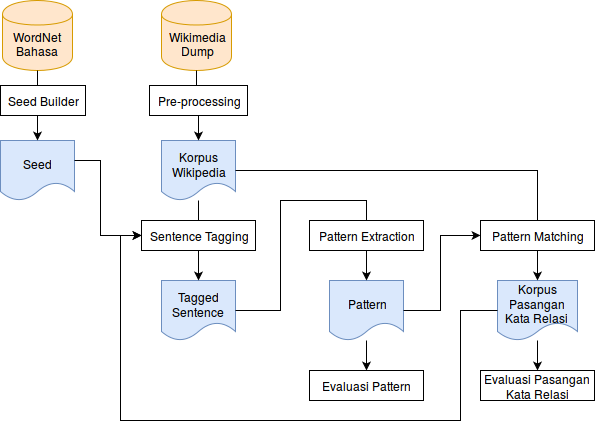
\includegraphics[scale=0.55]{pics/Pic01-SemiSupervisedCycle}
    \caption{Arsitektur Penelititan}
    \label{fig:arsitektur-penelitian}
\end{figure}

\noindent Berikut adalah penjelasan singkat setiap tahapan pada gambar di atas.
\begin{enumerate}
  \item \textit{Pre-processing} data \\
  Sebelum memulai penelitian, terdapat dua hal utama yang perlu dilakukan yaitu pengumpulan \textit{seed} dan pembentukan kalimat Wikipedia. Pengumpulan \textit{seed} dilakukan untuk mendapatkan pasangan kata relasi yang digunakan sebagai dasar penelitian. Proses ini memanfaatkan \textit{resource} yang dimiliki WordNet Bahasa. Selanjutnya, artikel Wikipedia yang diperoleh dalam bentuk \textit{Wikipedia dump} perlu diolah sehingga memiliki representasi sesuai dengan format yang diharapkan. Informasi yang diperlukan hanya bagian isi artikel dan ditulis dalam bentuk kalimat untuk setiap baris.
  \item Pembentukan \textit{pattern} \\
  Menggunakan \textit{seed} dan korpus kalimat Wikipedia, dilakukan \textit{tagging} pasangan kata berelasi terhadap kalimat-kalimat yang ada. Kalimat yang mengandung pasangan kata berelasi akan ditandai dan disimpan sebagai dasar proses selanjutnya. Kalimat-kalimat yang sudah di-\textit{tag} dengan pasangan kata berelasi kemudian akan digunakan untuk proses \textit{pattern extraction}. Hasil dari proses ini adalah sejumlah \textit{pattern} leksikal terbaik dari banyak \textit{pattern} unik yang dihasilkan.
  \item Ektraksi pasangan kata relasi \\
  \textit{Pattern} yang dihasilkan digunakan untuk mengekstrak pasangan kata relasi baru dengan dibantu korpus Wikipedia dengan \textit{POS tag}. Proses \textit{pattern matching} dilakukan dengan mencocokkan kata-kata bebas dalam \textit{pattern} dengan kalimat, kemudian mengambil bagian yang menempati posisi \textit{tag} hipernim-hiponim. Pasangan kata yang dihasilkan masuk ke dalam korpus pasangan kata relasi hipernim-hiponim.
  \item \textit{Cycle semi-supervised} \\ 
  Korpus pasangan kata relasi yang terbentuk digunakan untuk iterasi selanjutnya sesuai dengan metode \textit{bootstrapping}. Proses iterasi dilakukan hingga jumlah pasangan kata relasi baru yang dihasilkan jenuh. Setelah satu eksperimen selesai, proses evaluasi dilakukan secara kolektif untuk mengetahui akurasi setiap data yang dihasilkan.
\end{enumerate}

\noindent Proses ini diharapkan dapat menghasilkan korpus pasangan kata relasi \textit{hyponym-hypernym} yang berkualitas baik dan berukuran besar.


%-----------------------------------------------------------------------------%
\section{Pre-processing Data}
%-----------------------------------------------------------------------------%
Proses inti dari penelitian ini, \textit{pattern extraction} dan \textit{matching}, memerlukan dua masukan utama yaitu sejumlah pasangan kata hipernim-hiponim (\textit{seed}) dan teks dokumen yang digunakan sebagai korpus. Pasangan kata hipernim-hiponim digunakan untuk proses pembentukan \textit{pattern} sementara teks dokumen digunakan untuk memperoleh pasangan kata baru. Karena belum ada korpus pasangan kata relasi hipernim-hiponim Bahasa Indonesia, perlu dibentuk \textit{seed} yang akan digunakan sebagai dasar pasangan kata hipernim-hiponim. Teks dokumen yang digunakan, yaitu Wikipedia, juga memerlukan pemrosesan sebelum menjadi masukan sistem.

%-----------------------------------------------------------------------------%
\subsection{Pembentukan Kalimat Wikipedia}
%-----------------------------------------------------------------------------%
Data Wikipedia yang diperoleh dari Wikimedia \textit{dumps} masih mengandung banyak \textit{tag} yang tidak digunakan pada penelitian ini seperti \textit{tag} \textit{id} dan \textit{revision}. Selain itu simbol-simbol khusus (\textit{markup}). Penelitian ini ingin mengekstrak \textit{pattern} dari \textit{free text}, sehingga format-format khusus tersebut perlu dibersihkan. Gambar \ref{fig:wiki-dump} menunjukan contoh data XML yang diperoleh dari Wikimedia Dump. Setelah data Wikipedia dibersihkan dari simbol-simbol tersebut, langkah selanjutnya adalah merepresentasikan korpus dalam bentuk kalimat. 

\begin{figure}
    \centering
    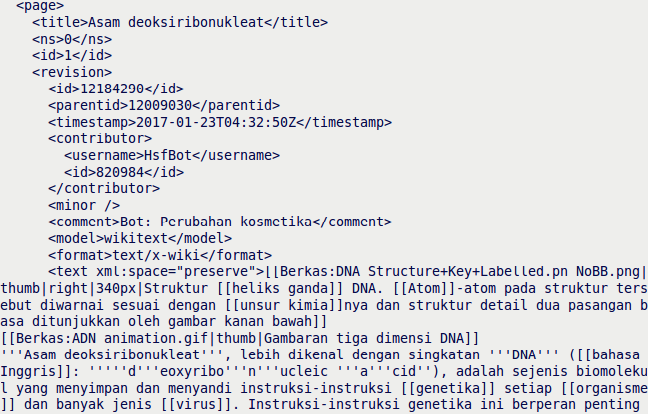
\includegraphics[width=\linewidth]{pics/WikipediaDump}
    \caption{Data XML Wikipedia Dump}
    \label{fig:wiki-dump}
\end{figure}

Artikel-artikel Wikipedia dibentuk ke dalam format yang telah didefinisikan dengan satu kalimat dipisahkan untuk setiap barisnya. Selanjutnya, data akan di format ulang sesuai definisi untuk mempermudah pemrosesan selanjutnya. Beberapa aturan yang diberikan adalah menghilangkan frasa di dalma tanda kurung, menghilangkan simbol, serta memberi \textit{tag start} dan \textit{end} pada awal dan akhir kalimat.

\begin{figure}
    \centering
    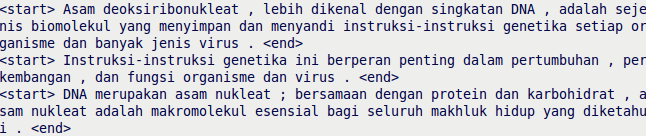
\includegraphics[width=\linewidth]{pics/kalimatWiki}
    \caption{Korpus kalimat Wikipedia tanpa \textit{POS tag}}
    \label{fig:kalimat-wiki}
\end{figure}

\begin{figure}
    \centering
    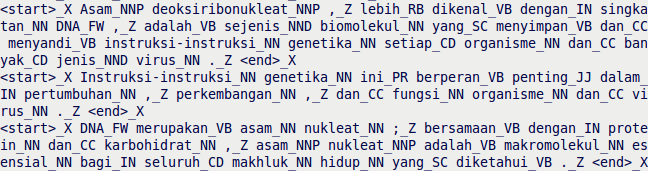
\includegraphics[width=\linewidth]{pics/kalimatWikiTag}
    \caption{Korpus kalimat Wikipedia \textit{POS tag}}
    \label{fig:kalimat-wiki-tag}
\end{figure}

\noindent Korpus kalimat yang dihasilkan kemudian digunakan untuk proses \textit{part-of-speech tagging}. Hasil dari \textit{pre-processing} data Wikipedia adalah dua korpus besar yaitu korpus kalimat tanpa \textit{POS tag} (Gambar \ref{fig:kalimat-wiki}) yang digunakan sebagai masukan \textit{pattern extraction} dan korpus kalimat dengan \textit{POS tag} (Gambar \ref{fig:kalimat-wiki-tag}) yang digunakan sebagai masukan \textit{pattern matching}. 

%-----------------------------------------------------------------------------%
\subsection{Pengumpulan Seed}
%-----------------------------------------------------------------------------%
Pasangan kata relasi hipernim-hiponim diambil dari data yang dimilki oleh WordNet Bahasa yang dikembangkan oleh NTU. Pemanfaatan WordNet Bahasa dilatarbelakangi jumlahnya yang lebih besar dibanding Indonesian WordNet (IWN). Relasi semantik antar kata pada WordNet Bahasa memanfaatkan WordNet Princeton versi 3.0. \textit{Synset} pada WordNet Bahasa dipetakan ke \textit{synset} WordNet Princeton, sehingga relasi semantik yang dimiliki oleh WordNet Princeton ikut diwarisi. Alasan lain penggunaan WordNet Bahasa adalah karena telah terintegrasi dengan \textit{tools} nltk sehingga dapat langsung digunakan untuk membentuk \textit{seed} secara mudah.

Seluruh lema Bahasa Indonesia yang ada di dalam korpus WordNet Bahasa diambil. Untuk setiap lema, akan dicari hipernimnya sehingga dapat dibentuk menjadi pasangan kata relasi hipernim-hiponim. Sayangnya, tidak semua pasangan kata yang dihasilkan adalah benar akibat beberapa kekurangan yang dimiliki WordNet Bahasa. Untuk itu dilakukan proses filterisasi untuk meminimalisasi \textit{error} yang mungkin terjadi. Dua tipe filterisasi yang digunakan adalah filterisasi lema sama dan filterisasi \textit{strict}. Filterisasi lema sama memperbolehkan pasangan kata terbentuk dari kata dengan \textit{synset} hiperim berbenda namun memiliki sejumlah lema yang sama. Sementara filterisasi \textit{strict} tidak memperbolehkan hal tersebut. Seluruh pasangan kata yang lolos proses filterisasi dibentuk menjadi \textit{tuple} biner. Hasil akhir dari proses ini adalah himpunan \textit{tuple} yang berisi dua elemen dengan format $(w_1;w_2)$ dimana $w_1$ pertama merupakan kata hiponim dan $w_2$ merupakan kata hipernimnya.

Beberapa contoh \textit{seed} yang dihasilkan adalah `(novel;buku)', `(salmon;ikan)', `(humus;tanah)', `(oktan;ukuran)', dan `(kucai;sayuran)'.


%-----------------------------------------------------------------------------%
\section{Pembentukan Pattern}
%-----------------------------------------------------------------------------%
\textit{Pattern} leksikal yang akan digunakan ingin seluruhnya dibentuk secara otomatis oleh sistem. Terdapat dua masukan utama untuk proses ini yaitu pasangan kata relasi hipernim-hiponim yang telah diketahui dan korpus dokumen. Pada tahap awal, pasangan kata relasi masukan adalah \textit{seed} yang dibentuk menggunakan WordNet Bahasa. Untuk tahap selanjutnya, pasangan kata relasi menggunakan korpus \textit{pair} hasil proses ekstraksi. Terdapat dua tahapan utama dalam pembentukan \textit{pattern} yaitu \textit{sentence tagging} dan \textit{pattern extraction}.

%-----------------------------------------------------------------------------%
\subsection{Sentence Tagging}
%-----------------------------------------------------------------------------%
\textit{Sentence tagging} adalah proses \textit{intermediate} yang perlu dilakukan sebelum sistem dapat membentuk sebuah \textit{pattern} leksikal. Proses ini akan memberi \textit{tag} hipernim dan hiponim terhadap suatu kata di dalam kalimat. Masukan untuk proses ini adalah pasangan kata relasi dan korpus Wikipedia tanpa \textit{POS tag}. Untuk setiap kalimat dalam korpus Wikipedia, dicek apakah kalimat tersebut mengandung pasangan kata relasi. Jika mengandung, maka kata dalam kalimat yang merupakan pasangan kata akan di-\textit{tag} hipernim dan hiponim. Satu kalimat dicocokan dengan seluruh pasangan kata relasi karena terdapat kasus dimana satu kalimat mengandung lebih dari satu pasangan kata relasi. Proses ini menghasilkan kalimat-kalimat Wikipedia yang telah diberi \textit{tag} hipernim atau hiponim.

Sebagai contoh, terdapat pasangan kata `(sepak bola;olahraga)' serta kalimat `{\tagStart} sepak bola adalah cabang olahraga yang menggunakan bola yang umumnya terbuat dari bahan kulit dan dimainkan oleh dua tim . {\fontfamily{qcr}\selectfont<end>}'. Kalimat dengan tag hipernim-hiponim yang dihasilkan adalah `{\tagStart} {\tagHyponym}sepak bola{\tagHyponymEnd} adalah cabang {\tagHypernym}olahraga{\tagHypernymEnd} yang menggunakan bola yang umumnya terbuat dari bahan kulit dan dimainkan oleh dua tim . {\tagEnd}'. Dengan adanya penanda kata mana yang merupakan hipernim dan hiponim, proses ekstraksi \textit{pattern} akan lebih mudah dilaksanakan.

%-----------------------------------------------------------------------------%
\subsection{Pattern Extraction}
%-----------------------------------------------------------------------------%
Setelah didapatkan kumpulan kalimat yang sudah diberi \textit{tag} hipernim dan hiponim, dicari barisan kata yang mirip dan dapat dijadikan sebuah \textit{pattern}. \textit{Pattern extraction} adalah proses untuk mendapatkan \textit{pattern} leksikal yang kemunculannya sering dalam korpus. Masukan dari proses ini adalah kalimat-kalimat Wikipedia yang telah diberi \textit{tag} hipernim dan hiponim. Dari kalimat tersebut akan dibuat suatu \textit{pattern tree} yang merepresentasikan seluruh \textit{pattern} leksikal yang ditemukan dan digunakan untuk mendapatkan \textit{pattern} yang paling sering muncul. Namun, tidak seluruh kata dalam kalimat akan dimasukkan ke dalam \textit{pattern tree}. Hanya bagian-bagian yang dianggap relevan saja yang digunakan untuk proses \textit{pattern extraction}. Pada tahap awal pengembangan, pemanfaatan seluruh kata dalam kalimat menghasilkan \textit{pattern} yang sangat banyak dan tidak umum. Sebagai contoh, proses \textit{sentence tagging} menghasilkan tiga kalimat yang telah diberi \textit{tag} hipernim-hiponim berikut. Kalimat digunakan untuk mencari \textit{pattern} yang merepresentasikan relasi hipernim-hiponim.
\begin{itemize}
  \item {\tagStart} {\tagHyponym}kelinci{\tagHyponymEnd} adalah {\tagHypernym}binatang{\tagHypernymEnd} yang gemar memakan wortel . {\tagEnd}
  \item {\tagStart} {\tagHyponym}mobil{\tagHyponymEnd} adalah {\tagHypernym}kendaaraan{\tagHypernymEnd} beroda empat . {\tagEnd}
  \item {\tagStart} selain sepak bola, {\tagHyponym}basket{\tagHyponymEnd} adalah {\tagHypernym}olahraga{\tagHypernymEnd} yang disukai masyarakat . {\tagEnd}
\end{itemize}
Dari kumpulan kalimat di atas, \textit{pattern} yang diinginkan untuk terbentuk adalah `{\tagHyponym} adalah {\tagHypernym}'. Sementara bagian seperti `gemar memakan wortel', `beroda empat', dan `yang disukai masyarakat' tidak merepresentasikan \textit{pattern} hipernim-hiponim. Hal tersebut memperlihatkan bahwa tidak seluruh kata dalam kalimat perlu dimasukkan ke dalam \textit{pattern tree}.

Berdasarkan hasil pengamatan secara kualitatif dari sejumlah kalimat yang telah diberi \textit{tag} hipernim-hiponim, terdapat tiga tipe pendekatan yang digunakan untuk proses pembentukan \textit{pattern}. Bagian dalam kalimat yang diperhatikan untuk pemebuatan \textit{pattern} adalah kata diantara dua \textit{tag} hipernim-hiponim, $n$ kata sebelum \textit{tag} pertama, dan $n$ kata setelah \textit{tag} terakhir. Bagian kata yang diambil akan dimasukkan ke dalam \textit{pattern tree} untuk mengetahui kemunculannya yang paling sering. Seluruh \textit{pattern} direpresentasikan menjadi vektor dan dirutkan berdasarkan bobot tertingginya. Proses ini akan menghasilkan kumpulan \textit{pattern} unik yang terurut berdasarkan bobotnya. Dari \textit{pattern} unik tersebut, akan diambil sejumlah \textit{pattern} terbaik untuk kemudian digunakan sebagai dasar pembentukan \textit{pair} baru. Lebih rinci mengenai proses pembentukan \textit{pattern} dapat dilihat pada bab 4.4.
%
% Sebagai contoh terdapat beberapa kalimat berikut.
% \begin{itemize}
%   \item {\tagStart} {\tagHyponym}piano{\tagHyponymEnd} adalah {\tagHypernym}alat musik{\tagHypernymEnd} yang dimainkan dengan cara dipukul . {\tagEnd}
%   \item {\tagStart} {\tagHyponym}komputer{\tagHyponymEnd} adalah {\tagHypernym}alat{\tagHypernymEnd} yang dipakai untuk mengolah data . {\tagEnd}
%   \item {\tagStart} {\tagHyponym}tupai{\tagHyponymEnd} adalah {\tagHypernym}mamalia{\tagHypernymEnd} yang mirip dengan bajing . {\tagEnd}
% \end{itemize}
%\noindent Dari kalimat di atas \textit{pattern} unik yang dihasilkan yaitu `{\tagHyponym} adalah {\tagHypernym}'. 


%-----------------------------------------------------------------------------%
\section{Ekstraksi Pair}
%-----------------------------------------------------------------------------%
Tujuan utama dari penelitian ini adalah membentuk korpus pasangan kata relasi, sehingga proses ekstraksi \textit{pair} adalah tahapan utama dari keseluruhan penelitian. Pada proses ini, dimanfaatkan \textit{pattern} yang telah terbentuk sebelumnya untuk mengekstrak pasangan kata baru. Pasangan kata tersebut kemudian difilter sebelum digabung ke dalam korpus pasangan kata relasi. Ektraksi \textit{pair} menggunakan teknik \textit{pattern matching}. Selanjutnya \textit{pair} akan diberi bobot dan hanya \textit{pair} yang bobotnya memenuhi nilai \textit{treshold}-lah yang akan dimasukkan dalam korpus pasangan kata relasi.

%-----------------------------------------------------------------------------%
\subsection{Pattern Matching}
%-----------------------------------------------------------------------------%
\textit{Pattern matching} adalah proses mencocokkan suatu \textit{pattern} ke dalam teks dokumen. Proses ini dilaksanakan untuk mendapatkan pasangan kata relasi (\textit{pair}) baru. Dua masukan utama untuk proses ini adalah \textit{pattern} dan korpus Wikipedia \textit{POS tag}. Penggunaan korpus Wikipedia dengan \textit{POS tag} untuk membatasi \textit{pair} yang terekestrak hanya berasal dari kelas kata benda (\textit{noun} atau \textit{proper noun}). Batasan ini karena relasi hipernim-hiponim umumnya digunakan untuk antar kelas kata benda dan untuk POS \textit{tag} yang digunakan, kedua \textit{tag} tersebut yang merepresentasikannya. Sayangnya, tidak seluruh \textit{pair} yang dihasilkan benar memiliki relasi hipernim-hiponim. Untuk itu, dihitung nilai bobot untuk seluruh \textit{pair} yang dihasilkan. Nilai bobot digunakan untuk dibandingkan dengan nilai threshold yang didefinisikan. Hanya \textit{pair} yang bobotnya melebihi nilai \textit{threshold} yang dapat masuk ke korpus pasangan kata relasi.

Sebagai contoh, terdapat \textit{pattern} leksikal `{\tagHyponym} adalah {\tagHypernym} yang'. Berikut adalah beberapa kalimat Wikipedia dengan \textit{POS tag}.

\begin{itemize}
  \item {\tagStart}\_X sepak\_NNP bola\_NNP adalah\_VB olahraga\_NN paling\_RB populer\_JJ di\_IN Britania\_NNP .\_Z {\tagEnd}\_X
  \item {\tagStart}\_X Berikut\_VB adalah\_VB daftar\_NN penghargaan\_NN yang\_SC diberikan\_VB .\_Z {\tagEnd}\_X
  \item {\tagStart}\_X Gado-gado\_NNP adalah\_VB makanan\_NN yang\_SC berasal\_VB dari\_IN Betawi\_NN .\_Z {\tagEnd}\_X
\end{itemize}

\textit{Pair} yang dihasilkan setelah melalui tahap \textit{pattern matching} hanya `(gado-gado;makanan)'. Pasangan kata `(berikut;daftar penghargaan)' tidak termasuk karena kata `berikut' bukan merupakan kata benda (\textit{noun}). Sementara walau `(sepak bola;olahraga)' adalah pasangan kata hipernim-hiponim yang benar, kalimat tersebut tidak cocok dengan \textit{pattern} leksikal yang diberikan menyebabkan \textit{pair} tidak terekstrak. Lebih rinci mengenai proses ekstraksi \textit{pair} dapat dilihat pada bab 4.5.

%-----------------------------------------------------------------------------%
\subsection{Pembobotan dan Filterisasi}
%-----------------------------------------------------------------------------%
Kumpulan \textit{pair} yang berhasil terekstrak tidak seluruhnya diterima ke dalam korpus pasangan kata relasi. Hanya \textit{pair} yang diyakini benar yang dapat masuk, untuk itu perlu dilakukan proses filterisasi. Setiap \textit{pair} akan diberi bobot dimana nilai bobot suatu \textit{pair} dihitung berdasarkan fitur-fitur yang dimiliki yang disimpan dalam bentuk vektor. Informasi utama dalam menghitung bobot suatu \textit{pair} adalah jumlah \textit{pattern} yang membentuk \textit{pair} tersebut serta nilai \textit{similariy} antara dua kata dalam \textit{pair}. Perhitungan jumlah \textit{pattern} pembentuk \textit{pair} dilakukan pada tahap \textit{pattern matching}. Sementara nilai \textit{similarity} dihitung menggunakan model \textit{word embedding}. Setiap \textit{pair} yang nilai bobotnya melebih nilai \textit{threshold} yang didefinisikan dapat masuk ke dalam korpus pasangan kata relasi.


%-----------------------------------------------------------------------------%
\section{Cycle Semi-Supervised}
%-----------------------------------------------------------------------------%
Pembelajaran menggunakan pendekatan \textit{semi supervised learning} dilatarbelakangi ketersediaan pasangan kata relasi semantik yang telah diketahui (\textit{seed}) berukuran terbatas dan korpus berukuran besar yang belum dianotasi. Ingin didapatkan \textit{pair} baru dari korpus yang belum diantoasi tersebut. Metode \textit{semi supervised} yang diterapkan adalah \textit{Bootstrapping}. Untuk lebih spesifiknya, algoritma \textit{bootstrapping} yang digunakan gabungan antara Meta-Bootstrapping dan Basilisk dengan beberapa modifikasi. Pemilihan metode tersebut didasari proses ekstraksi \textit{pair} baru yang memanfaatkan \textit{pattern}. Secara umum, proses \textit{bootstrapping} dikelompokan ke dalam dua tahap yaitu iterasi pertama dan iterasi ke-2 hingga n.

Pada iterasi pertama, proses pembentukan \textit{pattern} memanfaatkan \textit{seed} yang berasal dari WordNet Bahasa. Tahap \textit{pre-processing} menghasilkan kumpulan \textit{seed} dan korpus kalimat Wikipedia. \textit{Seed} digunakan untuk \textit{tagging} kalimat Wikipedia sehingga menghasilkan kalimat yang telah di-\textit{tag} hipernim-hiponim. Kalimat-kalimat tersebut digunakan untuk membentuk \textit{pattern} unik yang digunakan untuk memulai iterasi \textit{semi supervised}. \textit{Pattern} yang dibentuk dari filterisasi \textit{seed} lema sama maupun \textit{strict} digabung dan diurutkan berdasarkan bobot yang dimiliki. Lima \textit{pattern} terbaik diambil untuk selanjutnya digunakan dalam proses ekstraksi \textit{pair}. Sementara \textit{seed} yang membentuk kelima \textit{pattern} tersebut langsung dimasukkan ke dalam korpus pasangan relasi kata. Hal tersebut dilakukan untuk memfilter \textit{seed} salah yang terbentuk akibat \textit{error} dari \textit{resource} WordNet Bahasa. Selanjutnya, \textit{pattern} digunakan untuk mengekstrak \textit{pair} baru dan melakukan pembobotan terhadap \textit{pair}. Seluruh \textit{pair} yang nilai bobotnya melebihi \textit{threshold} bergabung dengan \textit{pair} dalam korpus pasangan kata relasi.

Iteriasi selanjutnya mirip seperti iterasi pertama yaitu melakukan \textit{tagging} pasangan kata relasi terhadapa korpus kalimat Wikipedia. Namun, untuk iterasi ke-2 hingga selanjutnya, pasangan kata yang digunakan untuk proses \textit{tagging} adalah dari korpus pasangan kata relasi semantik yang dihasilkan. Setelah mendapatkan kalimat yang telah di-\textit{tag} hipernim-hiponim, dilanjutkan dengan proses \textit{pattern extraction}. \textit{Pattern} yang dihasilkan akan digabung dengan seluruh \textit{pattern} lama kemudian diurutkan. Seperti pada metode \textit{Basilisk}, jumlah \textit{pattern} yang digunakan pada iterasi berikutnya akan bertambah. Satu \textit{pattern} terbaik dari hasil pengurutan bergabung dengan \textit{pattern} terpilih lama untuk digunakan dalam proses \textit{pattern matching}. Hal ini membuka kemungkinan adanya \textit{pair} baru terekstrak. Sama seperti proses sebelumnya, \textit{pair} yang bobotnya melebihi nilai \textit{threshold} digabung ke dalam \noindent pasangan kata relasi.

Iterasi dilakukan hingga korpus pasangan kata relasi jenuh atau dapat dikatakan \textit{pair} baru yang masuk ke dalam korpus berjumlah sedikit. Pada penelitian ini, jika \textit{pair} baru berjumlah kurang dari lima puluh maka iterasi akan berhenti. Evaluasi \textit{pattern} dan \textit{pair} dilakukan secara kolektif diakhir eksperimen. Anotator melakukan evaluasi secara manual untuk mengetahui kualitas \textit{pattern} dan \textit{pair} yang dihasilkan.


%-----------------------------------------------------------------------------%
\section{Metode Evaluasi}
%-----------------------------------------------------------------------------%
Penelitian ini tidak hanya menghasilkan korpus pasangan kata relasi hipernim-hiponim, namun juga \textit{pattern} leksikal Bahasa Indonesia yang merepresentasikan relasi tersebut. Setelah suatu eksperimen selesai, evaluasi dilakukan terhadap \textit{pattern} dan \textit{pair} yang dihasilkan. Proses evaluasi dilakukan dengan bantuan anotator.

%-----------------------------------------------------------------------------%
\subsection{Evaluasi Pattern}
%-----------------------------------------------------------------------------%
Evaluasi \textit{pattern} dilakukan dengan bantuan dua anotator dan melalui beberapa tahap. Berikut adalah proses yang dilakukan untuk evaluasi \textit{pattern}.
\begin{enumerate}
  \item Anotator membuat \textit{pattern} secara manual yang diyakini dapat mengekstrak kata-kata relasi semantik sesuai dengan format \textit{pattern} yang didefinisikan.
  \item Anotator melakukan penilaian terhadap \textit{pattern} yang dihasilkan oleh sistem. Suatu \textit{pattern} dinilai berdasarkan jumlah \textit{pair} benar maupun salah yang mungkin terekstrak dengan nilai antara 1 (sedikit), 2 (sedang), dan 3 (banyak).
  % \item Anontator melakukan \textit{ranking} dari \textit{pattern} hasil ekstraksi.
  \item Nilai \textit{precision} diperoleh dengan membandingkan \textit{pattern} yang dibentuk oleh anotator dan \textit{pattern} yang dihasilkan sistem.
  % \item Nilai Spearman's Rho diperoleh dengan membandingkan \textit{ranking pattern} yang dilakukan anotator dengan \textit{ranking pattern} yang dihasilkan sistem.
\end{enumerate}

\textit{Pattern} manual dibandikan dengan \textit{pattern} buatan sistem dengan melihat seberapa cocok keduanya. Suatu \textit{pattern} dapat dikategorikan ke dalam tiga kelompok yaitu, \textit{exact match}, \textit{partial match}, atau \textit{no match}. \textit{Pattern} dikatakan \textit{exact match} jika seluruh token dan urutannya dalam satu \textit{pattern} adalah tepat sama dengan \textit{pattern} yang lain. \textit{Pattern} dikatakan \textit{partial match} jika token dalam satu \textit{pattern} adalah subbagian dari keseluruh token untuk \textit{pattern} lainnya, dimana urutan kemunculan diperhatikan. Sebagai contoh, \textit{{\tagHypernym} adalah {\tagHyponym}} dan \textit{{\tagHypernym} adalah sebuah {\tagHyponym}} dapat dikatakan \textit{partial match}. \textit{Pattern} dikatakan \textit{no match} jika tidak memenuhi kriteria \textit{exact match} maupun \textit{partial match}.

\textit{Pattern} hasil sistem diberi nilai anotasi berdasarkan dua dimensi, yaitu banyaknya \textit{pair} benar yang dihasilkan dan banyaknya \textit{pair} salah yang dihasilkan. Anotator memberi nilai anotasi dengan skala 1 hingga 3, dimana nilai 1 berarti \textit{pair} berjumlah sedikit, nilai 2 berarti \textit{pair} berjumlah sedang, dan nilai 3 berarti \textit{pair} berjumlah banyak. Dari nilai anotasi, dibuat \textit{confussion-matrix} untuk diketahui banyaknya \textit{pattern} yang berkualitas tinggi. 
% Sementara \textit{ranking} yang digunakan anotator dibandingkan dengan \textit{ranking} yang dibuat sistem dan hasilnya dibandingkan.

%-----------------------------------------------------------------------------%
\subsection{Evaluasi Pair}
%-----------------------------------------------------------------------------%
Evaluasi \textit{pair} dilakukan menggunakan teknik \textit{random sampling}. Sejumlah \textit{pair} yang dihasilkan diambil secara acak dan dianotasi dengan nilai 'benar' atau 'salah' oleh anotator. Berikut adalah proses dalam evaluasi \textit{pair} hasil ekstraksi:
\begin{enumerate}
  \item Terdapat tiga anotator berbeda yang menganotasi data yang sama. 
  \item Anotator memberi nilai benar atau salah terhadap suatu \textit{pair} serta kategori yang didefinisikan. Untuk \textit{pair} benar dapat termasuk kategori \textit{pair} adalah \textit{instance-class} atau \textit{pair} adalah \textit{class-class}. Untuk \textit{pair} salah dapat termasuk kategori \textit{pair} tanpa relasi, \textit{pair} dengan relasi semantik lain, atau \textit{pair} yang posisi hypernym-hyponym-nya terbalik. 
  \item Nilai Kappa dihitung untuk mengetahui tingkat persetujuan antar anotator. Perhitungan dilakukan menggunakan Fleiss' Kappa.
  \item Hasil anotasi digunakan untuk menghitung akurasi \textit{pair} yang dihasilkan sistem.
\end{enumerate}

% TODO: tambahin penjelasan instance-class di bab 2 !!!
Dari setiap nilai anotasi, \textit{pair} dimasukkan ke dalam kategori yang lebih spesifik. Untuk data yang dianotasi benar, \textit{pair} dapat dimasukkan ke dalam dua kategori yaitu \textit{instance-class} atau \textit{class-class}. \textit{pair} dimasukkan ke dalam kategori instanace-class jika kata hyponym merupakan suatu instance, sementara kategori class-class jika kata hyponym merupakan suatu class. Untuk data bernilai salah, dapat dimasukkan ke kategori salah tanpa hubungan, salah akibat posisi hiponim-hipernim terbalik (\textit{false posistion}), atau salah dengan relasi semantik lain (\textit{false relation}). Kategori salah akibat posisi hiponim-hipernim terbalik terjadi saat kedua kata yang terekstrak benar memiliki relasi semantik hiponim-hipernim namun kata yang menempati posisi hiponim seharusnya adalah hipernim, begitu pula sebaliknya. Suatu \textit{pair} dapat digolongkan ke dalam kategori salah dengan relasi semantik lain jika kedua kedua kata dalam \textit{pair} tidak berhubungan hipernim-hiponim, namun memiliki relasi lain. Dalam penelitian ini, relasi lain hanya khusus dalam relasi semantik sinonim, antonim, atau meronym-holonym.

Akurasi \textit{pair} dihitung dengan melihat label benar atau salah yang diberikan oleh anotator. Jika terdapat perbedaan anotasi maka dilakukan \textit{voting} untuk menentukan label apa yang dipilih. Nilai akurasi dilihat terhadap seluruh eksperimen maupun setiap \textit{pattern} yang digunakan.
% Terdapat dua akurasi yang akan dihitung untuk setiap iterasi yaitu akurasi sampel dan akurasi total. Setiap iterasi menghasilkan \textit{pair} baru dan dari \textit{pair} baru tersebut diambil sampel untuk dianotasi. Nilai akurasi sampel adalah perbandingan antara data sampel baru benar dengan total data sampel baru. 
% \begin{equation}
% akurasi\,\,sampel = \frac{jumlah\,\,data\,\,sampel\,\,baru\,\,benar}{jumlah\,\,sampel\,\,baru}
% \end{equation}

% \noindent Sementara, akurasi total adalah perbandingan antara total data sampel bener dengan total data sampel.
% \begin{equation}
% akurasi\,\,total = \frac{jumlah\,\,total\,\,sampel\,\,benar}{jumlah\,\,total\,\,sampel}
% \end{equation}
